\chapter{Comparison study of CFD model and wind tunnel measurement}
\label{ch:wtcfdcomparison}
\def\figdir{chapters/ch07_wtcfdcomparison/figures}	

% description of the numerial method
% simulation domain description.
% boundary conditions
% how the leaf area density distribution is obtained
% comparison....
\section{Introduction}

\lettrine[lines=3,nindent=0em,loversize=0.1]{I}{n} this chapter, we compare the numerical method described in \cref{ch:parametricstudy} with the measurements of \cref{ch:microclimatestudy}. The measurements were performed for a small \textit{Buxus} \textit{sempervirens} plant. The measurements consisted of: i) X-ray tomography measuring plant microstructure metrics such as net leaf area and leaf area density, ii) stereoscopic particle image velocimetry (SPIV) measuring the wake flow characteristics such as mean velocity and turbulence kinetic energy (TKE), iii) infrared thermography measuring the spatiotemporal leaf temperature profile, and iv) hygrothermal in-foliage measurement probes measuring the vertical distribution of relative humidity (RH) and air temperature. Therefore, the goal of the present study is to compare the numerical simulation of the Buxus plant setup using the porous medium approach detailed in this thesis and compare with the high-resolution dataset to quantify the discrepancies. The present study aims at providing insight into the feasibility of employing such numerical techniques and possible limitations.

The fully-coupled numerical model described in \cref{ch:numericalmethod} is not used in this chapter for the comparison with the wind tunnel measurement. This is mainly because the measurement campaign detailed in \cref{ch:microclimatestudy}, although providing a high-quality measurement dataset of the air domain, still lacks necessary input parameters of the plant physiology such as CO$_2$ flux, stomatal conductance, xylem conductance, rhizosphere conductance, and the soil composition. It is recommended that to validate the full model, a more exhaustive measurement campaign should be designed measurements of air domain, soil domain, and plant physiology. Even with this limitation, the partial vegetation model,i.e., the air domain can be cross-examined with a real setup. Finally, we must note that as we use the simplified stomatal model described in \cref{ch:parametricstudy} in this chapter, hysteresis as observed in \cref{ch:microclimatestudy} cannot be modeled. This is because the stomatal resistance is only dependent on the atmospheric condition and not on the soil moisture content. 

\section{Simulation domain and boundary condition}

The simulation setup consisting of the numerical domain and its boundary conditions are that of the wind tunnel experiment with wind tunnel set wind speed $U_{\textit{ref}} = 1$ m\,s$^{-1}$. The reference velocity used for the study is the plant-canopy height velocity $U_h = 0.77$ m\,s$^{-1}$ at $H = 0.21$ m.

\subsection{Numerical domain}
	
	\begin{figure}[t]
		\centering
		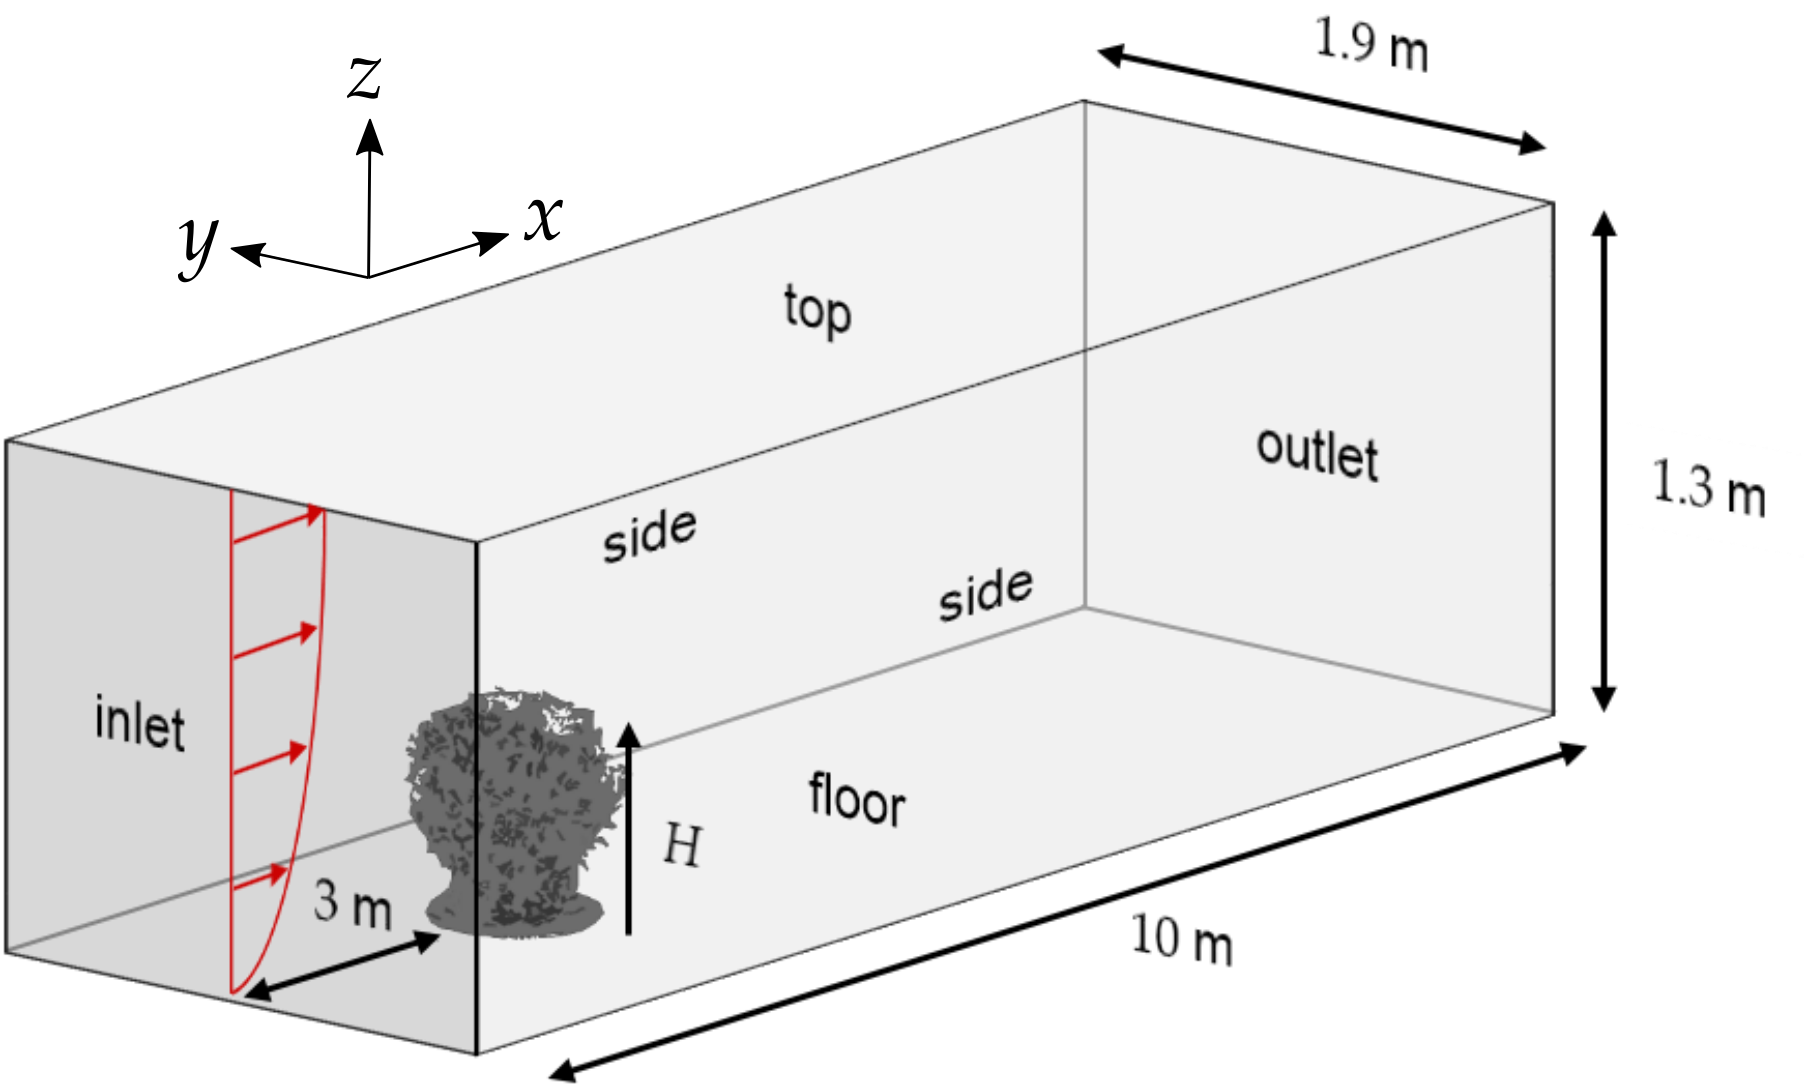
\includegraphics[width=0.8\textwidth]{\figdir/WT_CFD_comparison_setup_v3.png}
		\caption{Numerical domain used for the wind-tunnel-CFD comparison study with plant-canopy height $H = 0.21$ m (not to scale).}
		\label{fig:WT_CFD_comparison_setup}
	\end{figure}

The numerical domain is based on the geometry of the wind tunnel test-section with a wind tunnel height $H=1.3$ m and a lateral dimension $W=1.9$ m, as depicted in \cref{fig:WT_CFD_comparison_setup}. The upstream and downstream dimensions are chosen based on CFD best practices \citep{Blocken2015, Franke2007, Tominaga2008}. The inlet is located $15 H$ upstream from the plant, and the outlet is located at $32 H$ downstream from the plant, well above the recommended values of best practice guidelines. Thus, the downstream fetch of the numerical domain after the plant ensures a developed flow at the outlet of the numerical domain. Furthermore, the numerical scheme is also chosen to satisfy the best practice guidelines (see \cref{subsec:numericalsolution_wtcomp}). The numerical domain is discretized into $\num{413820}$ hexahedral cells with minimum cell size of $\num{7.81e-6}$ m$^{-3}$ (near the plant is present with a regular hexahedron) and a maximum cell size of $\num{2.2e-3}$ m$^{-3}$ at the top-outlet region. A grid refinement study was used to determine sufficient mesh resolution. The ground and lateral boundary $y^+$ are determined to be $37.9$ and $83.8$, respectively, satisfying the requirement for a valid wall function \citep{Franke2007}.


 %The plant frontal area is $A_{f} = 0.52$ m$^{2}$ and with a wind tunnel cross-sectional area of $A_{w}=3.04$ m$^2$, has a small blockage ration of $1.7$\%.

\subsection{Boundary conditions}

\begin{figure}[t]
	\centering
	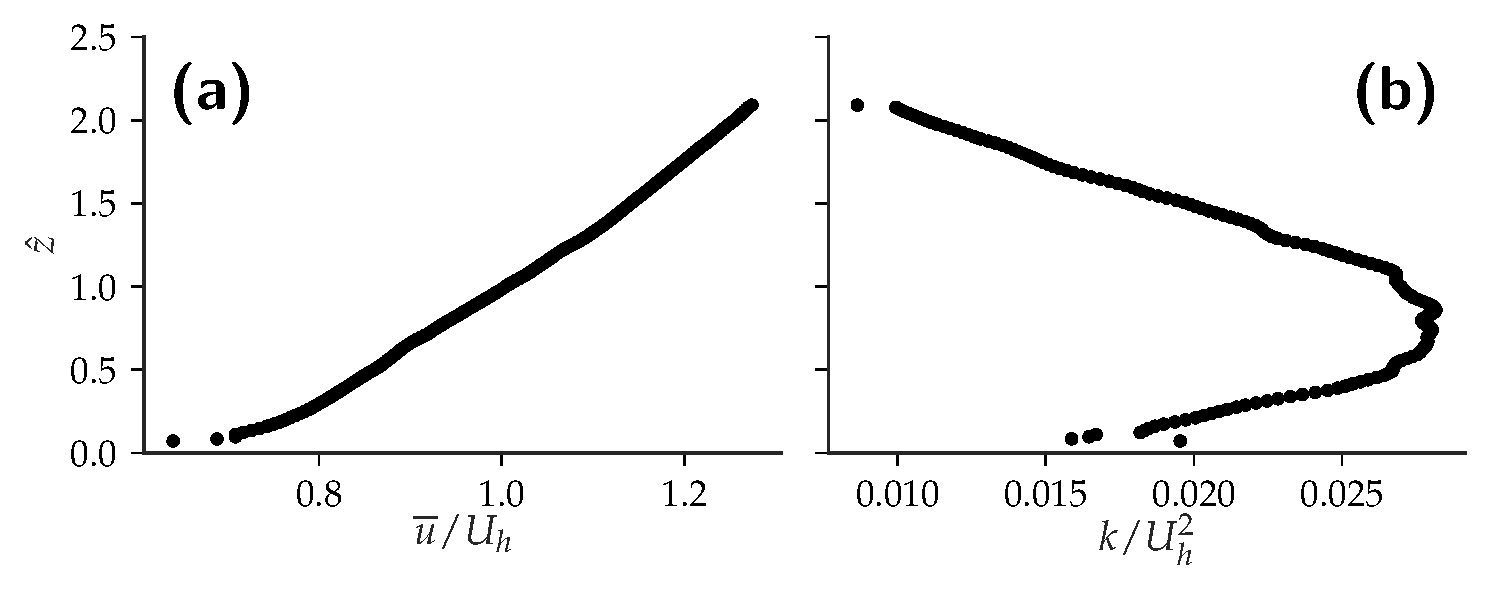
\includegraphics[width=0.8\textwidth]{\figdir/inletBoundarycondition_v2_inlettype2.pdf}
	\caption{Vertical profiles of incoming normalized \subfig{a} mean stream-wise velocity $\overline{u}/U_h$ and  \subfig{b} turbulent kinetic energy $k/U_h^2$ , obtained from PIV measurements.}
	\label{fig:boundaryprofile}
\end{figure}

\cref{fig:boundaryprofile} shows the inlet boundary condition of mean velocity $\overline{u}$ (m\,s$^{-1}$) and the turbulent kinetic energy $k$ obtained from the wind tunnel experiment, normalized with $U_h = 0.77$ m\,s$^{-1}$. The turbulent dissipation rate $\varepsilon$ is obtained through the atmospheric boundary layer (ABL) profile equations \citep{Richards1993}:
\begin{align}
	\tavg{u}(z) &= \frac{{{u_*}}}{\kappa }{\text{ln}}\left( {\frac{{z + {z_0}}}{{{z_0}}}} \right) \\
	k &= \frac{{{u_*}^2}}{{\sqrt {{C_\mu }} }} \\
	\varepsilon  &= \frac{{u_*^3}}{{\kappa \left( {z + {z_0}} \right)}}
	\label{eq:ableq}
\end{align}
where $\tavg{u}(z)$ (m\,s$^{-1}$) is the mean horizontal velocity, $u_*= \num{0.05052531}$ m\,s$^{-1}$ is  the friction velocity, $\kappa=0.41$ is von K\'arm\'an constant, $z_0 = \num{0.00133508}$ m is the aerodynamic roughness height and $C_{\mu}=0.09$. The inlet turbulent intensity is $I = \sqrt{2/3\,k}/U_{ref} = 12.1 \%$. The roughness height $z_0$ and the friction velocity $u_*$ is obtained using curve-fit of the measured PIV profile. The outlet boundary condition is defined as pressure outlet with a static pressure $p=0$. A zero-gradient boundary condition is enforced for $\mvec{u}$, $k$, and $\varepsilon$. The remaining boundaries (i.e., top-wall and side-walls) are modeled as no-slip wall-boundary and with standard wall functions.

\subsection{Vegetation: Leaf area density}

The vegetation is modeled as a porous medium parameterized using a leaf area density $a$ (m$^2$\,m$^{-3}$) distribution and a constant leaf drag coefficient $c_d$. For a detailed description, see \cref{sec:airdomain}. The source terms for momentum $\mvec{s}_u$ (N\,m$^{-3}$) , turbulence kinetic energy $s_k$ (W\,m$^{-3}$), and the turbulence dissipation rate $s_{\varepsilon}$ (W\,m$^{-3}$\,s$^{-1}$) are given as:
	\begin{align}
		\mvec{s}_u &=  - \rho {c_d}a\left| \tavg{\mvec{u}} \right|\tavg{\mvec{u}} 	\label{eq:source_veg1}	 \\
		s_k &= \rho {c_d}a\left( \beta _p \left| \tavg{\mvec{u}} \right|^3 - \beta _d\left| \tavg{\mvec{u}} \right|k \right) \label{eq:source_veg2} \\
		s_\varepsilon &= \rho {c_d}a\left( {{\beta _p}{C_{4\varepsilon }}{{\left| \tavg{\mvec{u}} \right|}^3}\frac{\varepsilon }{k} - {\beta _d}{C_{5\varepsilon }}\left| \tavg{\mvec{u}} \right|\varepsilon } \right)
		\label{eq:source_veg3}
	\end{align}
where $c_d$ is the leaf drag coefficient \citep{Wilson1977} and experimental measurements suggesting that $c_d \in \left[0.2, 0.5\right]$ \citep{Vogel1989}. The closure coefficients $C_{4\varepsilon}=0.9$ and $C_{5\varepsilon}=0.9$ are obtained from literature \citep{Katul2004, Kenjeres2013, Sanz2003}. The coefficients $\beta_p=1.0$ and $\beta_d=5.1$ are energy conversion ratio from MKE to TKE and TKE to heat, respectively. These parameters are dependent on the specific plant type and plant sample and would ideally require calibration. An insight to this is given in \cref{subsec:turbmodel}.

In this study, the X-ray tomography measured is used to determine the leaf area density $a$ distribution. Thereafter, the values are interpolated onto the numerical domain. A simple tri-linear interpolation scheme is employed to interpolate onto the finite volume cells. The leaf area density $a$ (m$^2$\,m$^{-3}$) is defined as the one-sided leaf surface area in a given volume and quantifies the spatial distribution of the vegetation in the environment. In our study, we determine the leaf area density $a$ using the porosity distribution measured in \cref{ch:microclimatestudy}: 
	\begin{equation}
	a = \frac{1}{2} A_l \frac{1 - \phi}{\int {1 - \phi }\,\mathrm{d}V}
	\label{eq:leafdensitywteq}
	\end{equation}
where $A_l$ (m$^{2}$) is the net plant leaf area (both sides of the leaves) and $\phi$ is the plant porosity. The leaf drag coefficient of $c_d = 0.5$ is chosen after the sensitivity study in \cref{subsec:dragcoeff}. It is seen to provide the closest prediction with the experimental measurements.

\subsection{Numerical solution}
\label{subsec:numericalsolution_wtcomp}
The problem is solved using the SIMPLE pressure-velocity coupling algorithm, obtaining a steady-state solution. The gradient terms are discretized using Gauss integration and interpolated using second-order central differenc\-ing sch\-eme (\texttt{linear}). Similarly, the divergence terms are interpolated using a second-order linear upwind differenc\-ing scheme (\texttt{linearUpwind}). The pressure is solved using geometric-algebraic multi-grid (GAMG) solver and preconditioned with diagonal incomplete-Cholesky (DIG) smoother, whereas velocity is solved using Preconditioned bi-conjugate gradient (PBiCG) solver with diagonal in\-comp\-lete-LU (DILU) pre\-conditioner. The matrix solvers are iterative\-ly solved until the residuals of pressure are below $\num{1e-5}$ and below $\num{1e-6}$ for all the other variables. Furthermore, under-relaxation factors are used with $\alpha_p = 0.3$ for pressure, $\alpha_u = 0.7$ for velocity (ensuring $\alpha_p + \alpha_u = 1$) and $\alpha_k = \alpha_{\varepsilon}=0.5$. The under-relaxation factors are modified to $\alpha_p=0.7$ and $\alpha_u=0.3$ when solving for non-iso\-thermal case to ensure stable convergence.

\section{Flow field}
\label{sec:flowfield}
In this section, the influence of the leaf area density distribution, plant drag coefficient, and the turbulence model is investigated. A preliminary assessment of the discrepancy between CFD and wind tunnel results is performed by comparing the mean velocity and TKE of the plant wake. Thereafter, the microclimate inside the plant is investigated by comparing the vertical profile of the air temperature and relative humidity for both the daytime and nighttime conditions (see \cref{sec:Microclimate}). A summary of parameters varied for the sensitivity study is given in \cref{tab:referencevalues}. The reference case values for drag coefficient, leaf area density distribution, and the turbulence model also indicated in \cref{tab:referencevalues}.


\ctable[
caption = {An overview of parameters varied in the sensitivity study along with the reference condition.},
label   = {tab:referencevalues},
mincapwidth = \textwidth,
pos = t,]{lll}{}{
	\FL
	Parameter							& reference                      & sensitivity study \\
	
	\ML
	drag coefficient  $c_d$				& $0.5$								   & $[0.2, 0.3, 0.4, 0.5, 0.6 ] $				                \\
	leaf area density $a$				& varying							   & constant vs. varying 	\\
	\multirow{2}{*}{turbulence model} & \multirow{2}{*}{por. real. $k-\varepsilon$} & [$k-\varepsilon$, real. $k-\varepsilon$, \\
	 																		& &		 por. $k-\varepsilon$, por. real. $k-\varepsilon$]	                
	\LL}

\begin{figure}[t]
	\centering
	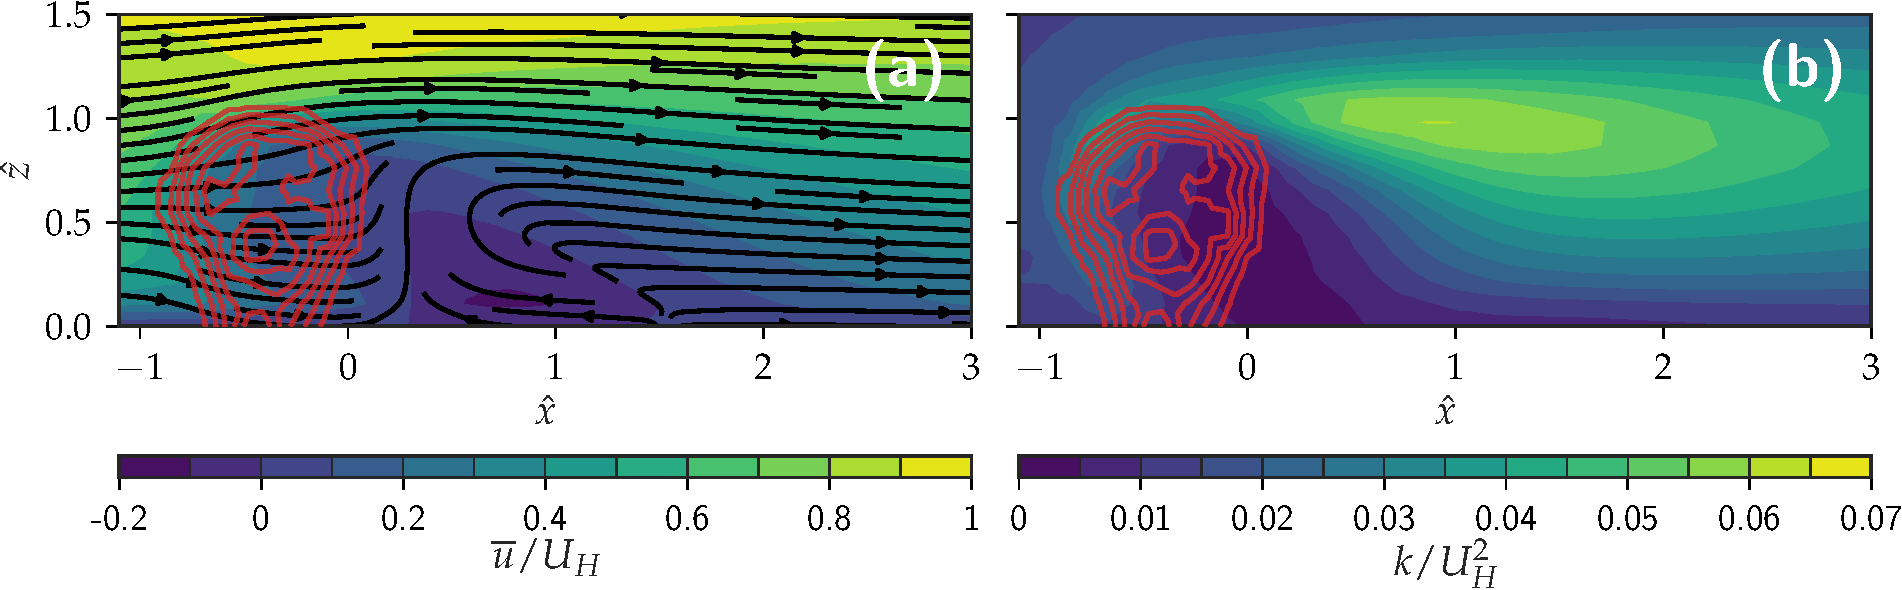
\includegraphics[width=\textwidth]{\figdir/basecase_vertical_UTKEstreamline_inlettype3-crop.pdf}
	\caption{Vertical plane at the center-line (i.e., at $\hat{y}=0$) from numerical simulation: \subfig{a} normalized  streamwise velocity $\overline{u}/U_H$ and \subfig{b} normalized  turbulent kinetic energy $k/U_H^2$ around the plant. The heterogeneous leaf area density $a$ is indicated with red iso-contour lines of $a = [20$, $40$, $60$, $80$, $100$, $120$, $140]$ m$^2$\,m$^{-3}$ and the drag coefficient is $c_d=0.5$.}
	\label{fig:basecase_vertical_UTKEstreamline}
\end{figure}

\cref{fig:basecase_vertical_UTKEstreamline} shows the stream-wise velocity $\overline{u}/U_H$ and TKE $k/U_H^2$ around (and within) the plant. The leaf area density is depicted using the iso-contour lines of $a = [20$, $40$, $60$, $80$, $100$, $120$, $140]$ m$^2$\,m$^{-3}$ determined using \cref{eq:leafdensitywteq}. It is seen to vary in space with peak density located approximately in the middle of the plant ($\hat{x}=-0.5$, $\hat{z}=0.5$). The velocity field is plotted together with the streamlines (\cref{fig:basecase_vertical_UTKEstreamline}a). The near-wake of the plant is consists of recirculation zone below $\hat{z} = 0.5$, indicated by negative stream-wise velocity. The highest TKE is observed at the plant-canopy height $\hat{z} = 1$, with peak TKE at approximately $\hat{x} = 1$. Therefore, the wake turbulence is seen to dominantly affected by the shear-zone generated by the plant canopy.

\cref{fig:basecase_horiz_U} show the normalized mean velocity magnitude at 8 horizontal planes where the PIV measurement were obtained in \cref{ch:microclimatestudy} as shown in \cref{fig:meanflow}. Additionally, the velocity field is plotted together with the streamlines. Comparing with experimental data, we see that both the numerical model and experiment measurement shows a recirculation zone behind the tree at $\hat{z}=$ [$0.29$,\,$0.43$]. However, at $\hat{z}= 0.57$ and $\hat{z}=0.71$, the numerical prediction deviates from the experimental observations. The complex streamlines as observed from experimental data are not present in the numerical simulation but instead show more of a bleed type of flow. Furthermore, the velocity deficit predicted by the simulation at $\hat{z}\le 1$ is slightly lower than in the experimental observation. This minor discrepancy can be attributed to the plant foliage is represented in the simulation. We have employed a porous media approach, where instead of directly representing the topology of the plant, we have parameterized it using leaf area density. Essentially, a spatial low pass filter has been applied to the plant topology and is represented by a density function. Such representation is known to comprise the prediction of spatial variability of the wake velocity statistics \citep{Endalew2009}.  

\begin{sidewaysfigure}[p]
	\centering
	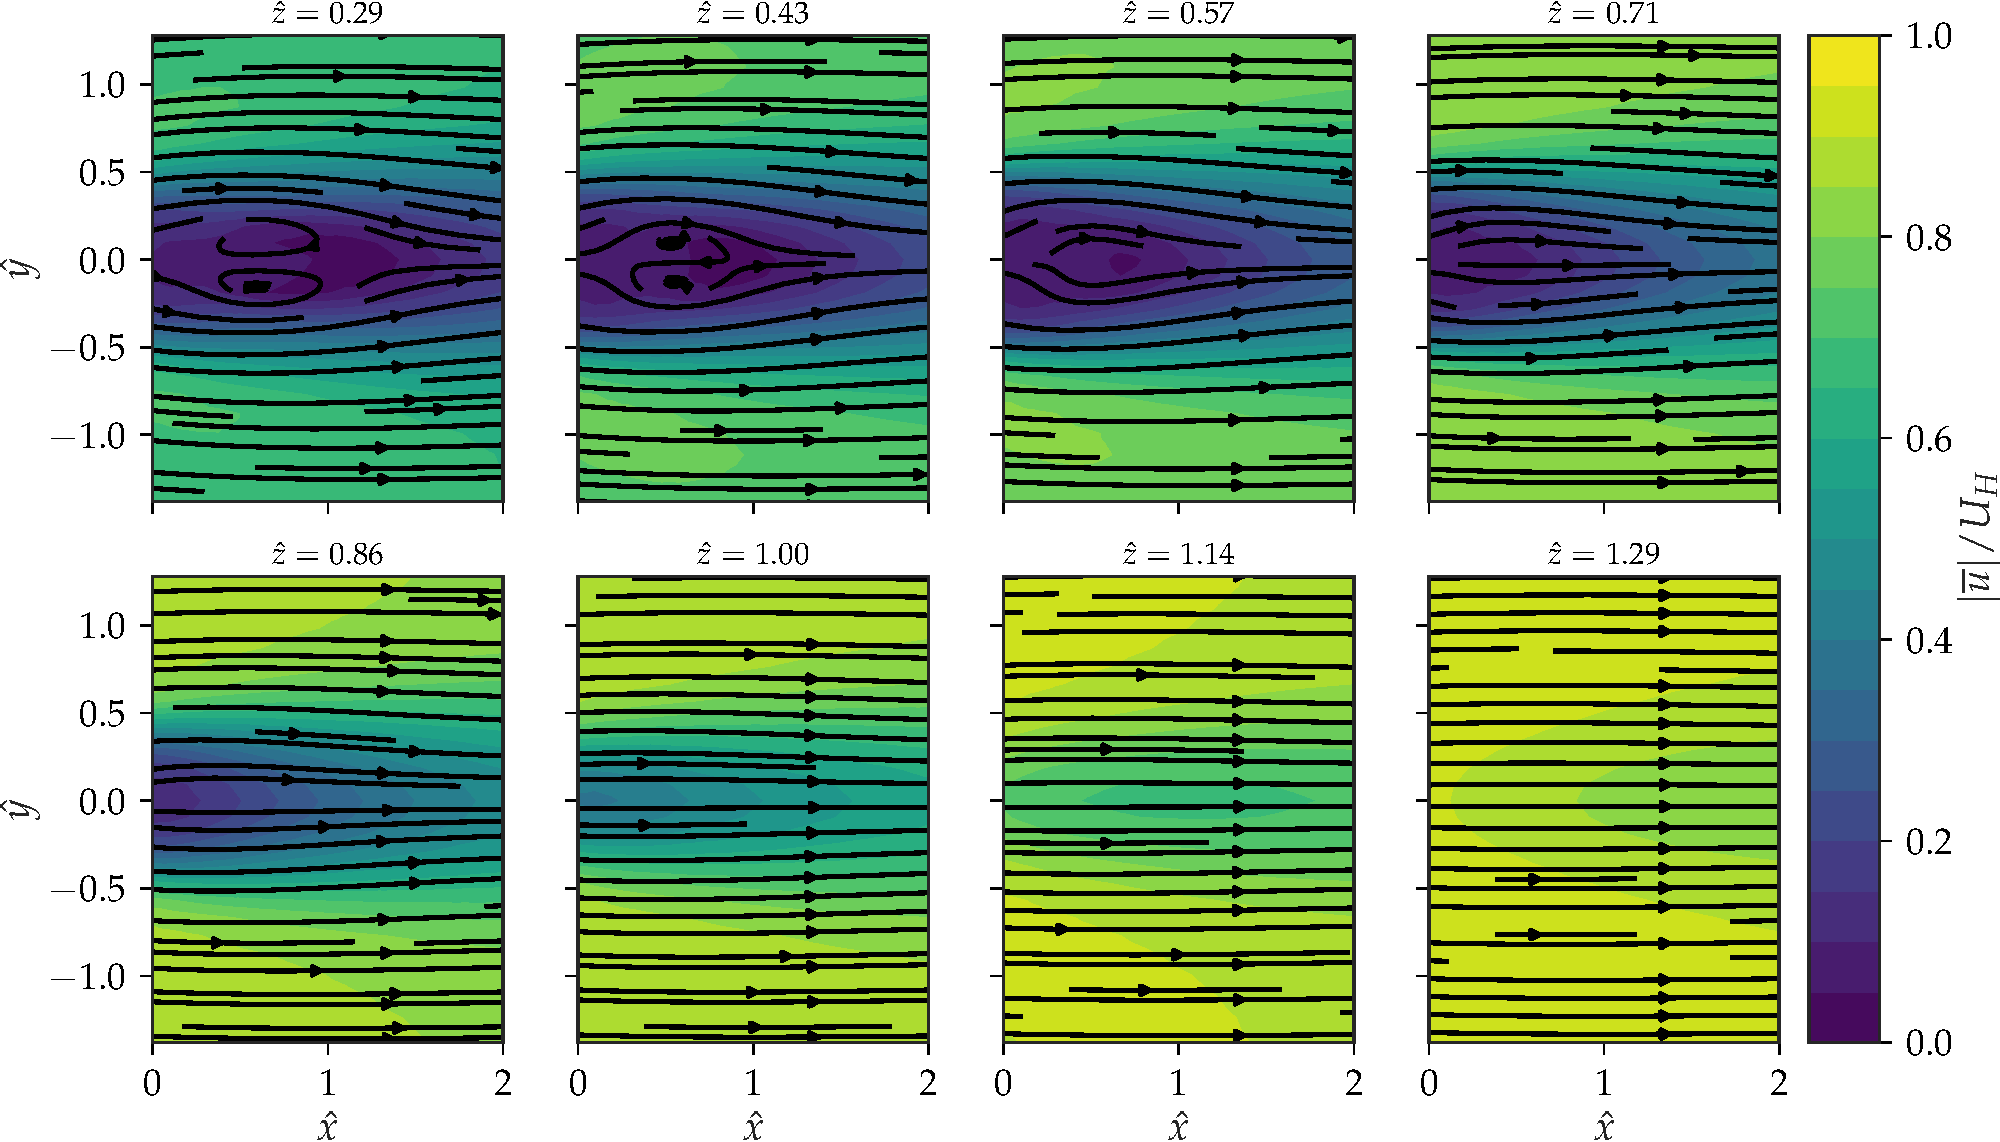
\includegraphics[width=\textwidth]{\figdir/basecase_horiz_U_inlettype3-crop.pdf}
	\caption{Normalized mean velocity magnitude $|\tavg{\mvec{u}}|/U_H$ at 8 horizontal planes, $\hat{z}=$ [$0.29$,\,$0.43$,\,$0.57$, $0.71$, $0.86$, $1.0$, $1.14$, $1.29]$. The experimental results of the same location at shown in \cref{fig:meanflow}.}
	\label{fig:basecase_horiz_U}
\end{sidewaysfigure}


\begin{sidewaysfigure}[p]
	\centering
	%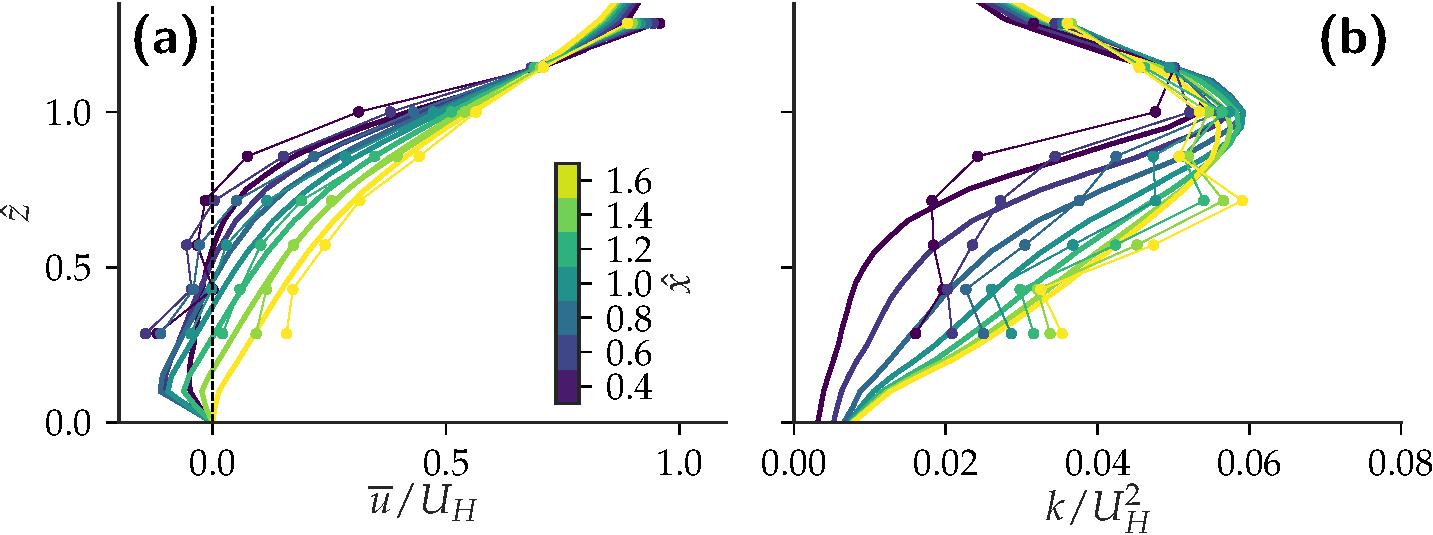
\includegraphics[width=\textwidth]{\figdir/basecase_horizprofile_UTKE_inlettype3-crop.pdf}
	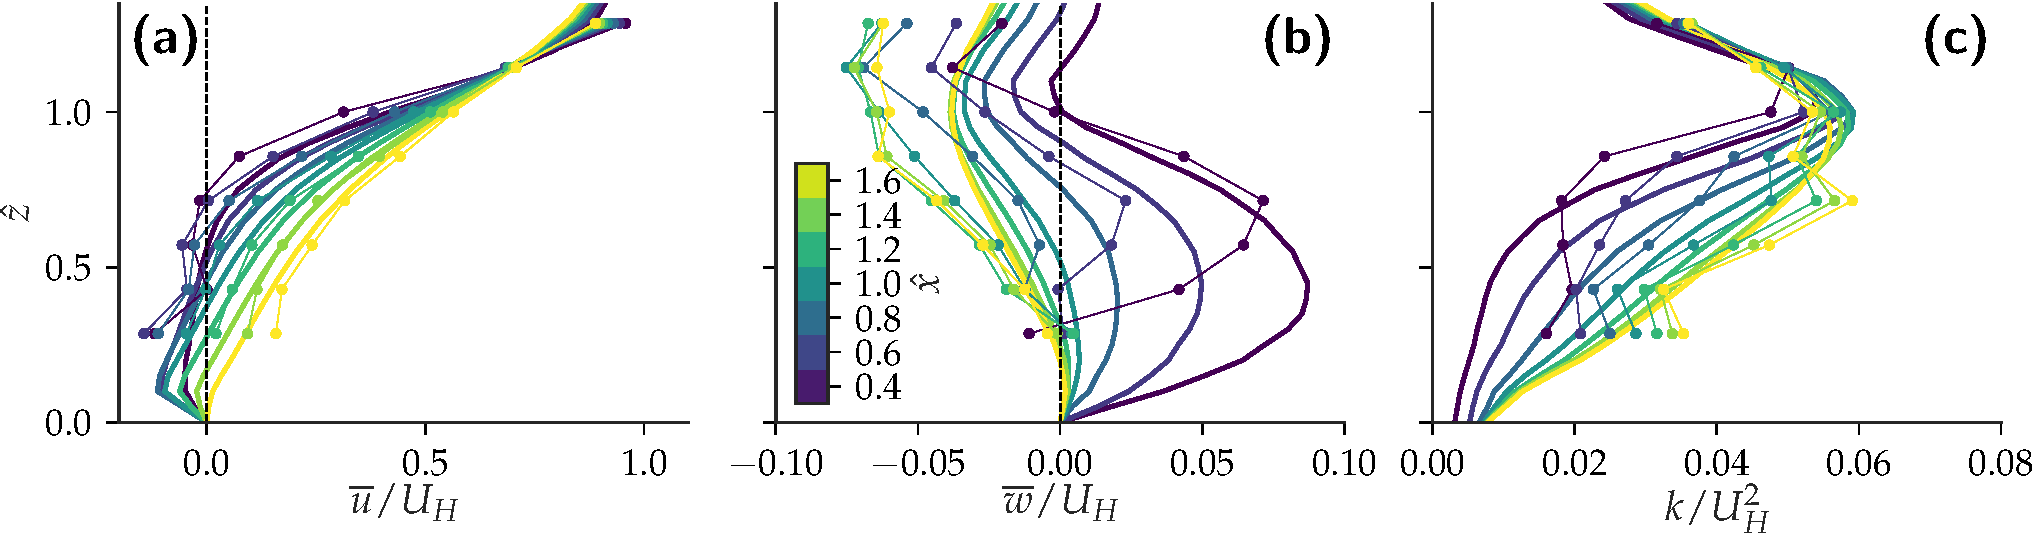
\includegraphics[width=\textwidth]{\figdir/basecase_horizprofile_UWTKE_inlettype3-crop.pdf}
	\caption{Mean vertical profiles at 7 streamwise positions $\hat{x}$, at center-line of the plant $\hat{y} = 0$: \subfig{a} streamwise velocity $\overline{u}/U_H$, \subfig{b} vertical velocity $\overline{w}/U_H$\subfig{b} turbulent kinetic energy $k/U_H^2$. The numerical and experimental results (obtained from \cref{fig:verticalprofile}) are plotted using solid smooth (---) and marked line ($-\bullet-$), respectively.}
	\label{fig:basecase_horizprofile_UTKE}
\end{sidewaysfigure}


\begin{figure}[p]
	\centering
	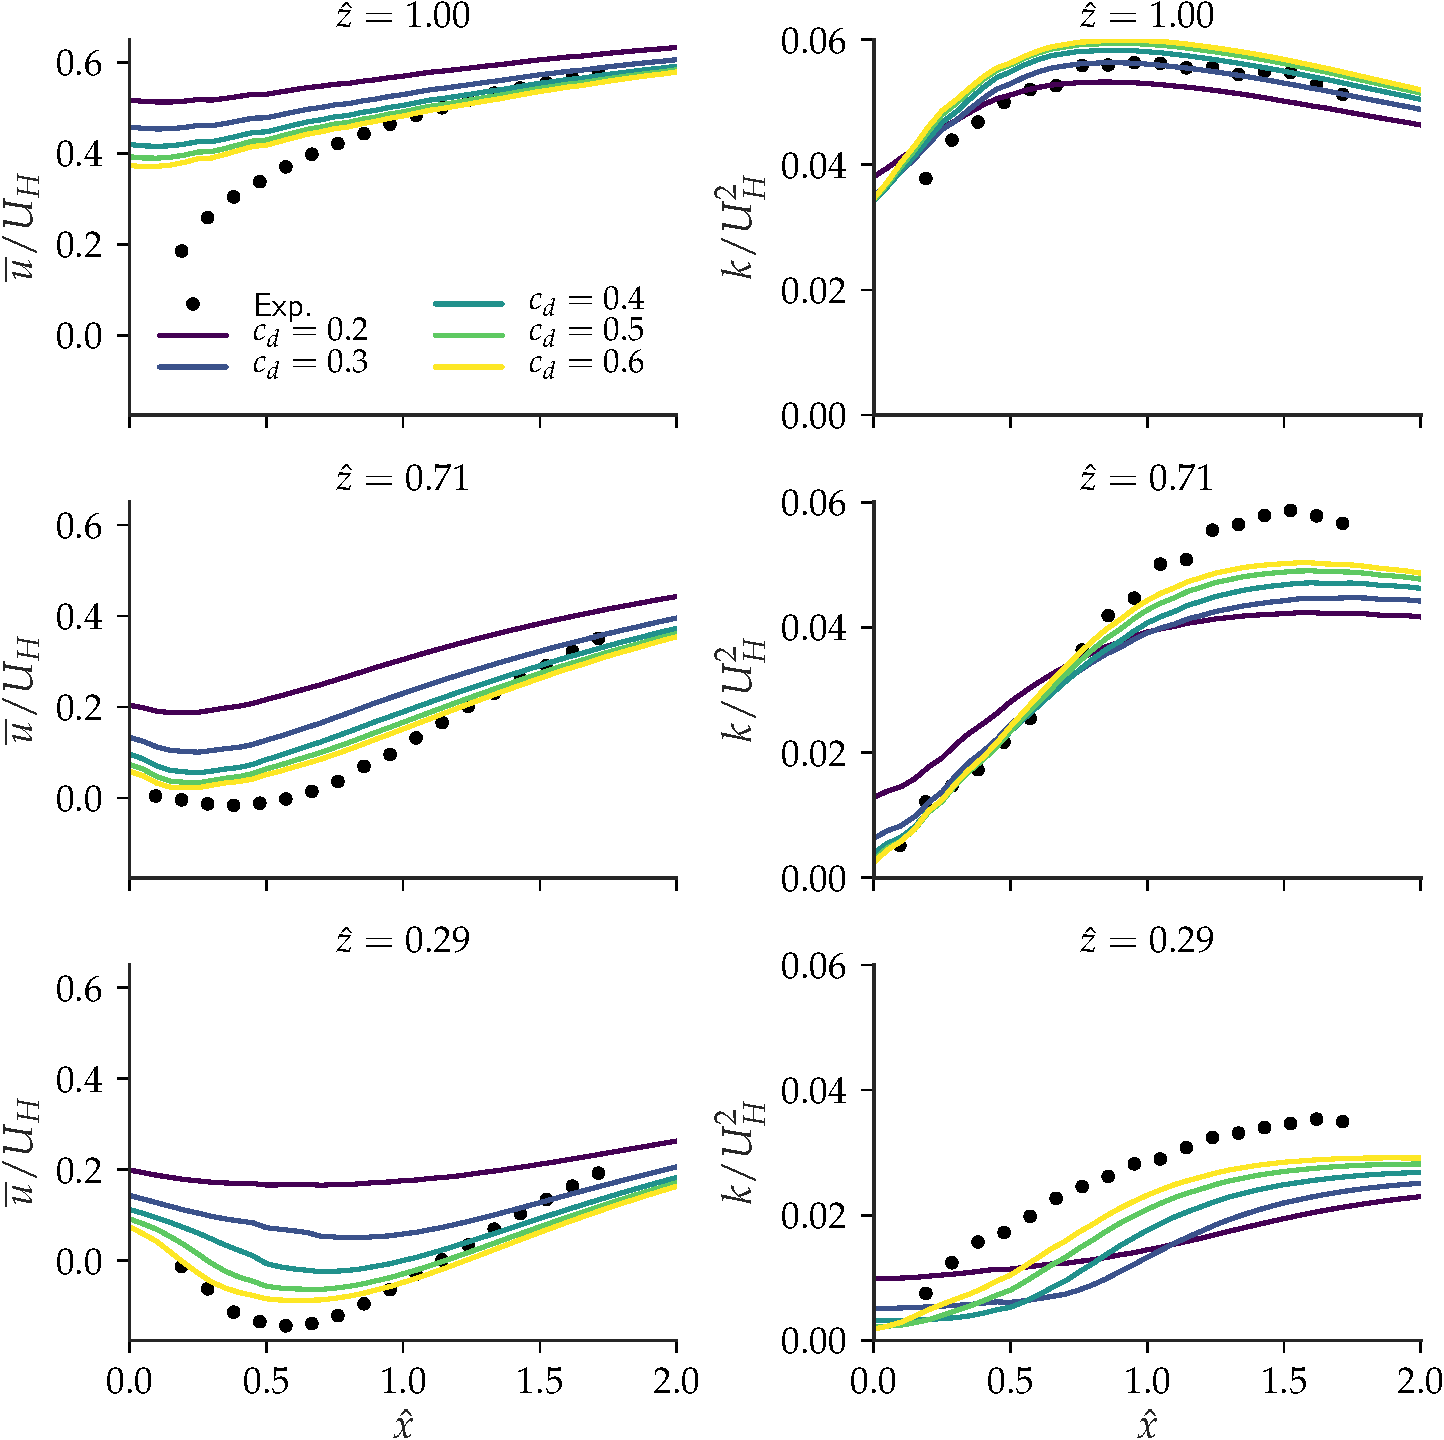
\includegraphics[width=\textwidth]{\figdir/WTvsCFD_cd_inlettype3-crop.pdf}
	\caption{Influence of drag coefficient $c_d = [0.2$, $0.3$, $0.4$, $0.5$, $0.6]$: Horizontal profile of normalized stream-wise velocity $\overline{u}/U_H$ and turbulent kinetic energy $k/U_H^2$ at heights $\hat{z} = [0.29$, $0.71$, $1]$ and $\hat{y}=0$.}
	\label{fig:WTvsCFD_cd}
\end{figure}

A preliminary comparison of the numerical prediction and the experimental measurement is performed by comparing the stream-wise velocity and the TKE at $\hat{x} = [0.4$, $0.6$, $0.8$, $1.0$, $1.2$, $1.4$, $1.6]$. \cref{fig:basecase_horizprofile_UTKE} shows the vertical profiles at these seven locations, where the lateral position is at the plant center-line (i.e., $\hat{y} = 0$).  The comparison shows a reasonable prediction of the near-wake statistics of the plant. The prediction especially demonstrates a good prediction of the magnitude and the gradient of the stream-wise velocity. However, the largest discrepancy is for the vertical velocity $\overline{w}$, very close to the tree $\hat{x} < 0.6$. The numerical model predicts a large updraft near the ground and under-predicts the downdraft downstream of the plant. Similarly, very close to the tree, $\hat{x} < 0.6$, the deficit in the velocity is seen to be under-predicted. The TKE shows a good comparison as well with an accurate prediction of the peak TKE at the plant-canopy shear-layer. However, as with the stream-wise velocity, very close to the tree, there is a slight overestimation. Furthermore, the variation over height is seen to less apparent than the experimental observation. This is most likely due to the numerical approach being a porous media approach where instead of explicitly resolving the plant elements (i.e., branches and leaves), they are aggregated into a distribution function.

\subsection{Influence of drag coefficient}
\label{subsec:dragcoeff}
A second plant property that determines the net influence of the vegetation on the flow is the drag coefficient $c_d$ in \crefrange{eq:source_veg1}{eq:source_veg3}. Generally, the drag coefficient is associated with the leaf drag coefficient and determined to be  $c_d \in [0.2, 0.5]$ \citep{Vogel1989,Wilson1977}. However, as there is a high quantity of branch elements in the small Buxus plant, the validity of the assumption is investigated by a parametric study on the drag coefficient.

\cref{fig:WTvsCFD_cd} shows the horizontal profile of  stream-wise velocity and turbulent kinetic energy at three heights $\hat{z} = [0.29$, $0.71$, $1]$ and $\hat{y}=0$, and the influence of drag coefficient on them. We observe clearly that the numerical prediction approaches to the experimental results as $c_d$ increases. Therefore, there is a clear indication that the drag coefficient of the plant is not just that of the leaf but should also take into account the contribution of the remaining plant elements such as branches. Thus, a drag coefficient of $c_d = 0.5$ is chosen as it not only provides a very good prediction accuracy, but is also within the constraint of  $c_d \in [0.2, 0.5]$ \citep{Vogel1989,Wilson1977} even though we observe that $c_d=0.6$ provides a slightly better prediction. However, the wake velocity deficit still shows a slight under-prediction. Similarly, in the wake zone (i.e., $\hat{z} < 1$), the peak TKE is under-predicted. 

\subsection{Influence of heterogeneity in leaf area density distribution}

\begin{figure}[p]
	\centering
	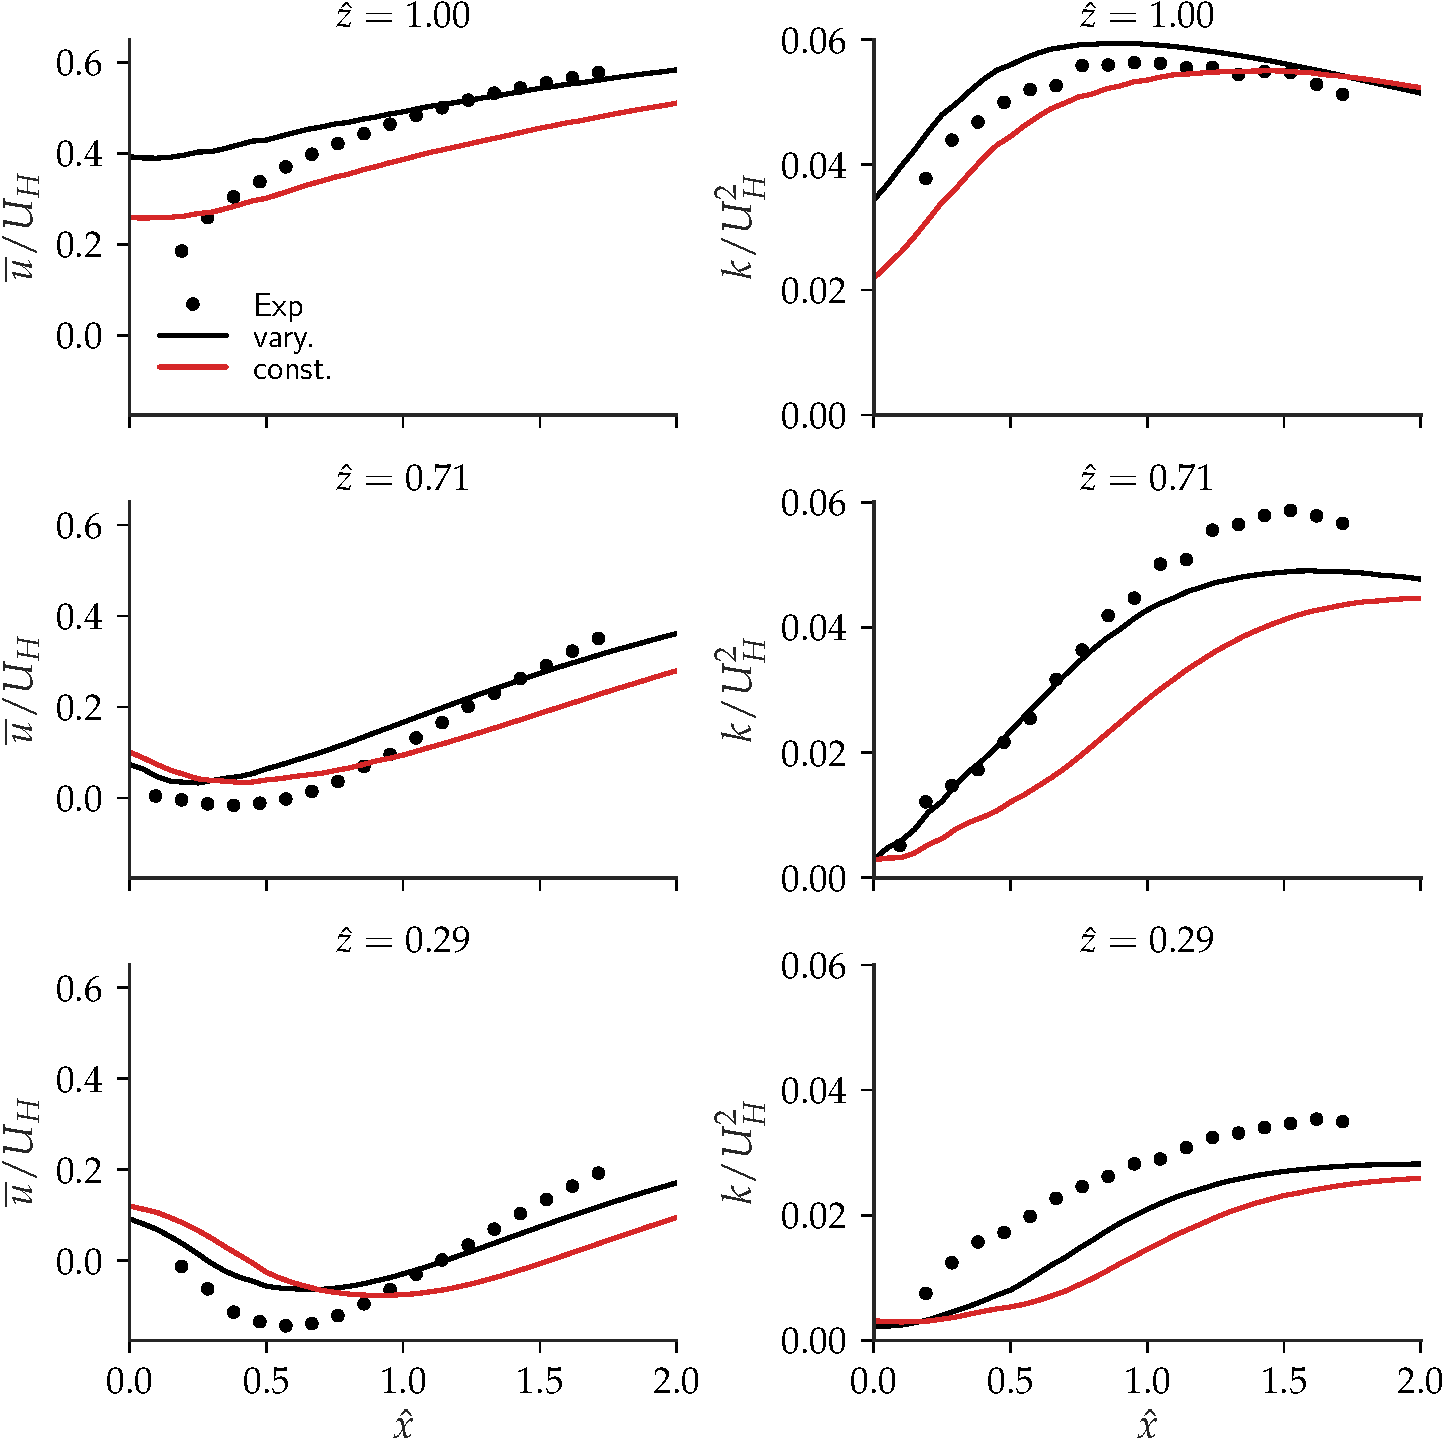
\includegraphics[width=\textwidth]{\figdir/WTvsCFD_LAD_inlettype3_nearest-crop.pdf}
	\caption{Influence of constant and varying leaf area density $a$ (m$^2$\,m$^{-3}$): Horizontal profile of stream-wise velocity $\overline{u}/U_H$ and turbulent kinetic energy $k/U_H^2$ at heights $\hat{z} = [0.29$, $0.71$, $1]$ and $\hat{y}=0$.}
	\label{fig:WTvsCFD_LAD}
\end{figure}

The influence of heterogeneity in the leaf area density distribution is investigated by comparing a spatially \textit{varying} leaf area density and a spatially \textit{constant} (average) leaf area density. Applying a spatial averaging operator to \cref{eq:leafdensitywteq}, we obtain the average leaf area density $\langle a\rangle$  (m$^2$\,m$^{-3}$) as:
	\begin{equation}
	\langle a \rangle = \frac{1}{2} {A}_l \frac{1 - \langle \phi \rangle}{\int {1 - \phi }\,\mathrm{d}V}
	\label{eq:leafdensitywteqaverage}
	\end{equation} 
where it is simply related to net leaf area $A_l$ and the average plant porosity $\langle \phi \rangle$. Therefore, the \textit{constant} leaf area density distribution in the air domain $\Omega_a$ is defined:
\begin{equation}
a(\mvec{x}) =
	\begin{cases}
	\langle a \rangle       	  & \quad \text{if}\ 0\le \phi < 1\\
	0  							  & \quad \text{if}\ \phi = 1
	\end{cases}
	\label{eq:leafdensitywteqaveragefield}
\end{equation}

\cref{fig:LAD_constvsvarying} shows the two types of leaf area density distribution at $\hat{y} = 0$. A spatially-averaged leaf area density is seen to be around $\langle a \rangle \approx 80$ m$^{2}$\,m$^{-3}$, with maximum leaf area density $\max (a) = 140$ m$^{2}$\,m$^{-3}$. %Due to the interpolation of the leaf area density from the initial measurement dataset to the finite volume grid, the leaf area distribution is seen to have a blurring effect at the edges. 

% However, due to the mesh discretization, the leaf area density distribution of \textit{constant} is seen to ``diffused'' (or ``blurred'') at the interface of the plant region. With increased mesh resolution, this edge-effect can be overcome.
	
\begin{figure}[t]
	\centering
	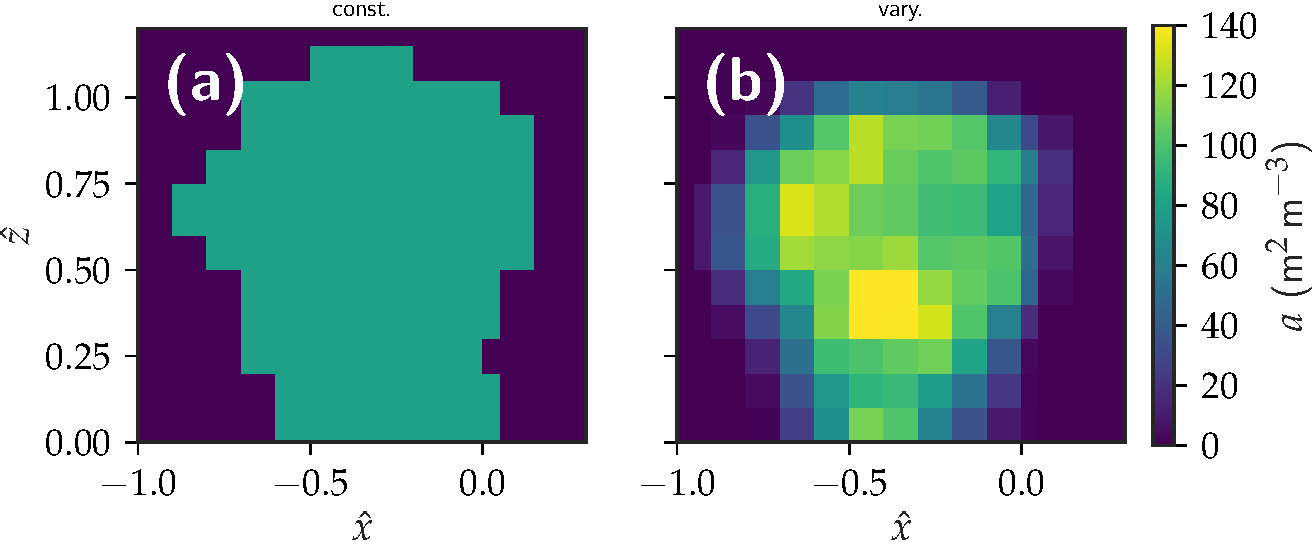
\includegraphics[width=\textwidth]{\figdir/LAD_constvsvarying_v2_nearest-crop.pdf}
	\caption{Two types of leaf area density $a$ distribution: \subfig{a} constant distribution and \subfig{b} varying distribution.}
	\label{fig:LAD_constvsvarying}
\end{figure}

To study the impact of heterogeneous leaf area density distribution, both cases are compared with the wind tunnel measurements. \cref{fig:WTvsCFD_LAD} shows the horizontal profile of  stream-wise velocity and turbulent kinetic energy at three heights $\hat{z} = [0.29$, $0.71$ $1]$.  The figure reveals that both constant and varying leaf area density distribution shows similar behavior where the more realistic description of the varying leaf area density distribution is seen to provide better predictions. The stream-wise velocity profile shows that the numerical model under-predicts the peak wake velocity deficit at all heights. Furthermore, the wake recovery from the numerical model is seen to be slower than the measurements. Therefore, the recirculation length of the numerical model is seen to be larger than in reality. One of the possible contributing factors to the recirculation length is the accuracy of the turbulence closure. Therefore, the influence of the turbulence model is investigated in more detail. 

\subsection{Influence of turbulence model}
\label{subsec:turbmodel}
	
	\begin{figure}[p]
		\centering
		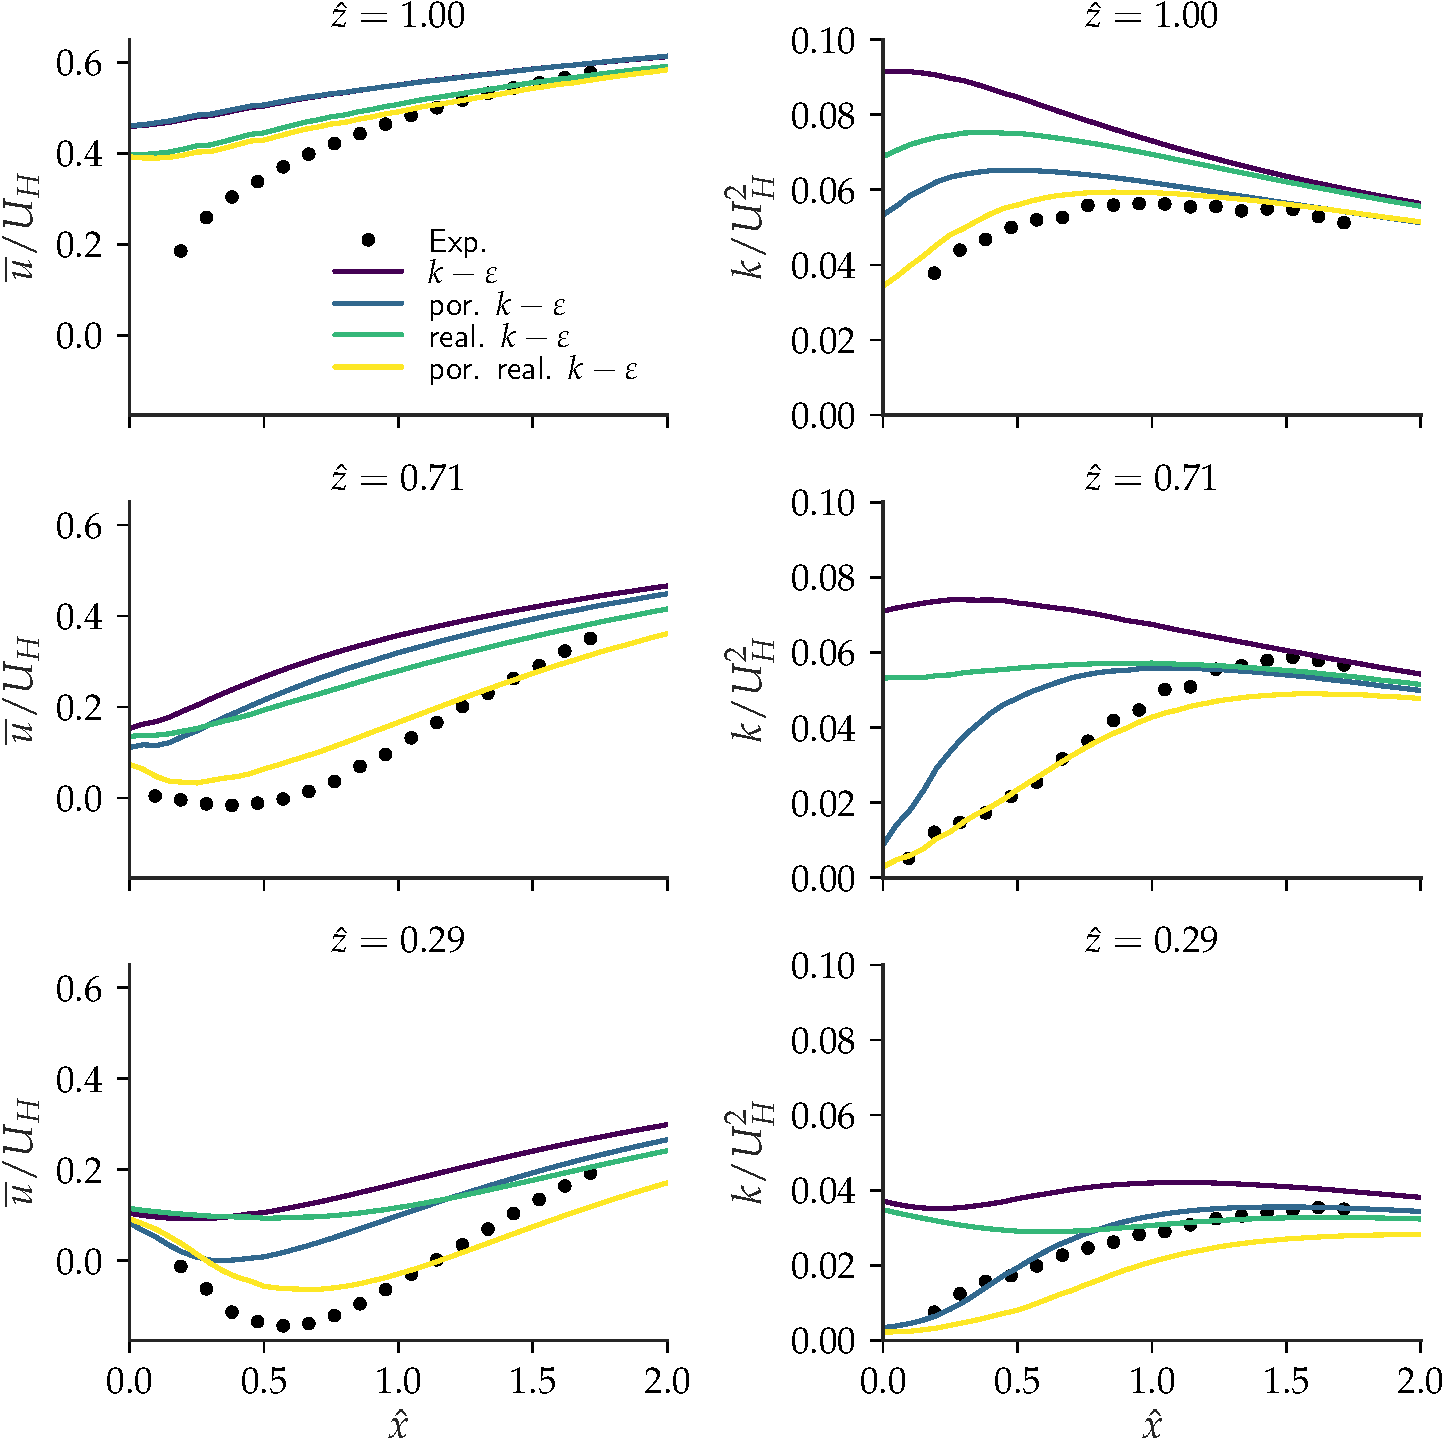
\includegraphics[width=\textwidth]{\figdir/WTvsCFD_RASModel_inlettype3-crop.pdf}
		\caption{Influence of turbulence model std. $k-\varepsilon$, std. real. $k-\varepsilon$, por. $k-\varepsilon$ and por. real. $k-\varepsilon$: Horizontal profile of normalized stream-wise velocity $\overline{u}/U_H$ and turbulent kinetic energy $k/U_H^2$ at heights $\hat{z} = [0.29$, $0.71$, $1]$ and $\hat{y}=0$.}
		\label{fig:WTvsCFD_RASModel}
	\end{figure}
		
For the study of the turbulence model, four similar closure approaches were investigated: i) $k-\varepsilon$, ii) realizable $k-\varepsilon$, iii) porous $k-\varepsilon$, and iv) porous realizable $k-\varepsilon$. The porous turbulence models (i.e., por. $k-\varepsilon$ and por. real. $k-\varepsilon$) have been modified with additional source terms, i.e., \cref{eq:source_veg1,eq:source_veg2,eq:source_veg3}, which models the influence of vegetation on the flow turbulence. 

\cref{fig:WTvsCFD_RASModel} shows the influence of the four turbulence closure approaches on the stream-wise horizontal profile of stream-wise velocity $u$ and turbulent kinetic energy $k$ at three heights $\hat{z} = [0.29$, $0.71$ $1]$. The study shows the clear importance of an accurate turbulence closure to obtain the real observed plant wake. Let us first look at the influence of the turbulence model by comparing $k-\varepsilon$ and realizable $k-\varepsilon$. We see that this change already has a good improvement of the numerical prediction. The realizable turbulence model is seen to outperform the $k-\varepsilon$ model providing more realistic velocity deficit and reduces the overestimation of the TKE. However, we see that the turbulence closure terms of the vegetation have a significantly stronger impact on the accuracy of the prediction. With the addition of vegetation source terms (i.e., por. $k-\varepsilon$ and por. real. $k-\varepsilon$), the models are seen to perform drastically better than the standard models. We see that, not only is the wake velocity deficit more pronounced as with observation, but the TKE at the vicinity of the plant is seen to be less over-predicted. Therefore, the impact of foliage, such as the TKE suppression from the fluid-structure interaction of the foliage and airflow, is seen to be an important aspect of vegetation. As the standard turbulence models do not model such shortcuts in turbulence cascade (i.e., from TKE to heat), an over-prediction of turbulence is observed. The best performance in prediction accuracy is seen to be obtained from the porous realizable $k-\varepsilon$ model, where the stream-wise velocity deficit and the magnitude of the TKE are predicted with good accuracy. However, at the plant-canopy height (i.e., $\hat{z} = 1$), very close to the foliage (i.e., $\hat{x} \rightarrow 0$), the strong plant wake velocity deficit is not captured. This could be fundamentally due to the shortcomings of a porous media and similar immersed boundary approach where boundary layer flow phenomena are weakly captured. The flow characteristics prevalent the interfaces such as shear-flow are no longer captured with such spatial definition and intensity. In future, the present study on the influence of the turbulence model can be expanded to investigate additional eddy-viscosity models such as $k-\omega$ or $k-\omega$ SST, Reynolds stress models (RSM), or even Large-eddy simulation (LES) . A more complex, computationally expensive turbulence modeling approach has been shown to improve the prediction accuracy \citep{Hiraoka2011,Yue2008,Lopes2013}. However, it is currently out of scope for the the present thesis but can potential be a topic for for future research.

An additional aspect of the turbulence closure is the model coefficients such as $c_{\mu}$, $C_{1\varepsilon}$, $C_{2\varepsilon}$, $C_{4\varepsilon}$, $C_{5\varepsilon}$, $\beta_p$ and $\beta_d$. These are also typically referred to as \textit{free} coefficients and typically requires rigorous calibration (i.e., tuning) to capture and recover the experimental observations. The calibration of these coefficient to the experiment results can be described as an optimization problem \citep{Margheri2014, Duraisamy2018, Couplet2005, Najm2009, Lucor2007, Gorle2015a}, where data assimilation techniques are well regarded as an effective methodology to ensure the accurate, efficient convergence to global optima:
\begin{equation}
\mathop {\arg \min }\limits_{\mvec{c}}\ \epsilon(\mvec{x}, \mvec{c}) = \left\| {\mathcal{N}(\mvec{x}) - \mathcal{M}(\mvec{x},\mvec{c})} \right\|_2 
\end{equation}
where $\mvec{c}=({{c_\mu },{c_{1\varepsilon }},{c_{2\varepsilon }},{c_{4\varepsilon }},{c_{5\varepsilon }},{\beta _p},{\beta _d}})^T$ is a vector of the free coefficients and $\mvec{c}$ spans $\mathbb{R}^7$, $\mathcal{N}$ is the true Navier-Stokes solution (neglecting the experimental uncertainties) and $\mathcal{M}$ is the numerical model. Therefore, the numerical model can be regarded as a ``black-box'' simply dependent on the free coefficient vector $\mvec{c}$. We see that a brute-force search for coefficient vector $c$ that minimizes the error $\epsilon$ is intangible as the search needs to be formed in a 7-dimensional space, requiring a rigorous search algorithm. Therefore, the calibration of the turbulence model is beyond the scope of the study, but an important aspect for future studies. 

\section{Microclimate}
\label{sec:Microclimate}

Finally, the numerical prediction of the thermal impact of the plant is compared with the hygrothermal wind tunnel measurements with ambient conditions $T = 21$ $^{\circ}$C, $25$\% relative humidity and plant-canopy incident solar radiation levels $q_{\textit{r,sw}} = \left[0,\ 100\right]$ W\,m$^{-2}$. To study the hygrothermal conditions, the temperature and humidity equations are solved where the additional plant source is determined using the leaf energy balance approach described in \cref{ch:parametricstudy}. Additionally, the resistance-based aerodynamic and stomatal models described in the chapter are used to parameterize the heat and mass flux between the foliage and air. The minimum stomatal resistance of the plant is set to $r_{\textit{s,min}} = 400$ s\,m$^{-1}$ (in \cref{eq:rs}), a typical value for deciduous plants \citep{Baille1994,Bruse1998}. Furthermore, it is equivalent to a stomatal conductance of $k_{\textit{st}} = 40$ mmol\,m$^{-2}$\,s$^{-1}$ (see \cref{eq:ksteff} ), typical of a \textit{Buxus} \textit{sempervirens} \citep{Rodriguez-Calcerrada2013a,Letts2012}. In our study, the characteristic plant leaf size is set to $l=3$ cm, obtained from measurements.

\begin{figure}[t]
	\centering
	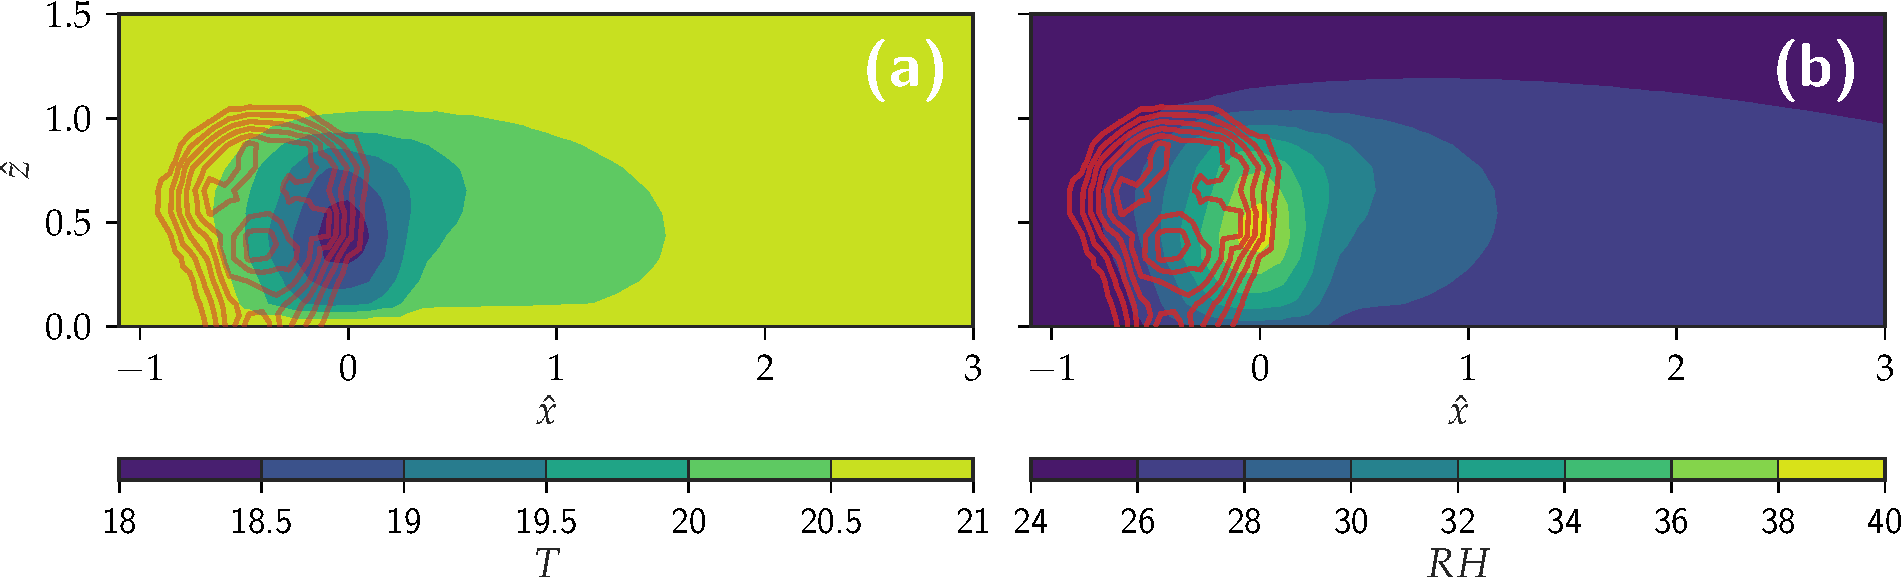
\includegraphics[width=\textwidth]{\figdir/vert_hygrothermal_plane_inlettype3-crop.pdf}
	\caption{Center-plane (i.e., $y=0$) hygrothermal condition of the flow at day-time with $T = 21$ $^{\circ}$C, $\textit{RH}=25$\% and $q_{\textit{r,sw,0}} = 100$ W\,m$^{-2}$: \subfig{a} air temperature $T$ ($^{\circ}$C) and \subfig{b} relative humidity $\mathit{RH}$ (\%).}
	\label{fig:vert_hygrothermal_plane}
\end{figure}


\cref{fig:vert_hygrothermal_plane} shows the temperature and relative humidity at the center-plane of the plant ($y=0$) during day time. A peak temperature drop of approximately $\Delta T = -2.5$ $^{\circ}$C and humidity rise of $\Delta RH = +12$\% is observed near the mid-aft region of the plant ($\hat{x} = 0$, $\hat{z} = 0.5$). We also note that there is no observed heating of the flow, typically present at the plant canopy height, possibly due to the lower level of incident solar radiation $q_{\textit{r,sw,0}} = 100$ W\,m$^{-2}$ and high convective heat transfer arising from the presence of wind. 

To accurately assess the discrepancy between the hygrothermal prediction and the experiment observation, the in-foliage air temperature, and relative humidity are compared at various vertical locations. \cref{fig:figure_airtemperature_relativehumidity_profile2} shows the vertical profile of the air temperature and relativity humidity during day and night where the results of the numerical simulation are plotted with dashed lines. At night, the hygrothermal parameters are well predicted with a minimal discrepancy. During the day, we see that there is an overestimation of the transpirative cooling. It is indicated by lower air temperature and higher relative humidity as respect to the experimental observations. This discrepancy is observable at the mid-foliage region (i.e., $\hat{z} = 0.5$) where the largest transpirative cooling is predicted. In contrast, the experimental results do not indicate a large cooling, maintaining a relatively similar air temperature during both day and night. Therefore, the discrepancy is associated with the overestimation of the transpiration by the plant foliage in the simulation. Inside the foliage, the maximum discrepancy between the numerical model and the experimental measurements is seen be small with approximately $0.5$ $^{\circ}$C and $2\%$ difference in air temperature and relative humidity, respectively. 

However, the high air temperature at the plant-canopy at seen in experimental measurements is not observed in the numerical prediction. The experimental observations, \cref{ch:microclimatestudy}, showed that air temperature is due to solar radiation interception at the top region of the foliage resulting in an increase in air temperature. At this location, the air temperature discrepancy between the numerical model and the experimental measurements is seen to be high, approximately $1.5$ $^{\circ}$C. In the simulation, the excess radiation absorption and the resulting rise in air temperature is not observed. The discrepancy could be possible due to the porous medium approach of resolving the plant foliage. As the plant canopy region is not explicitly resolved and instead described by plant density distribution, the strong radiative absorption that is present is not captured accurately. 

\begin{figure}[t]
	\centering
	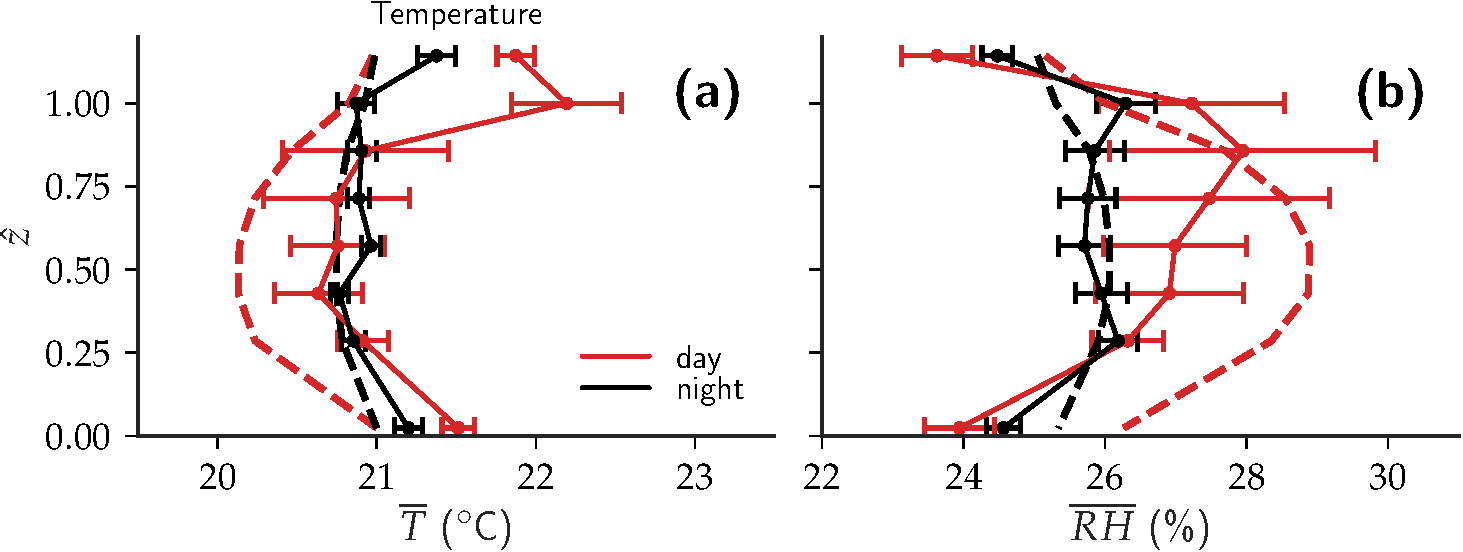
\includegraphics[width=\textwidth]{\figdir/figure_airtemperature_relativehumidity_profile_inlettype3-crop.pdf}
	\caption{Comparison of wind tunnel (solid, ---) and numerical simulation (dashed, $--$): \subfig{a} median air temperature $T$ ($^{\circ}$C) and \subfig{b} median relative humidity $\mathit{RH}$ (\%). Vertical distribution are divided into day ($08$:$00$ - $16$:$00$) (red) and night ($20$:$00$ – $04$:$00$) (black).}
	\label{fig:figure_airtemperature_relativehumidity_profile2}
\end{figure}

A more general assessment on the prediction of the plant transpiration can be assessed by examining the net plant transpiration rate during day and night. \cref{tab:nettranspirationcomp} shows the experimental and numerical value of the net transpiration rate $\textit{TR}$ (g\,h$^{-1}$) during day and night. The comparison validates the finding that numerical model predicts a high transpiration rate. Especially during the daytime, a very high transpiration rate of $17.1$ g\,h$^{-1}$ is predicted in contrast to the mean transpiration rate of $5.8$ g\,h$^{-1}$ and a peak transpiration rate of $14.8$ g\,h$^{-1}$. During the night, the net transpiration rate is predicted to be $4.9$ g\,h$^{-1}$, and the experimental observation suggests a mean and peak value of $3$ and $8.6$ g\,h$^{-1}$, respectively. The numerical prediction of the plant transpiration is quite similar to the maximum plant transpiration rate. This indicates that time-dependent stomatal regulatory phenomena, as observed in chapter \ref{ch:microclimatestudy} is not captured as we have employed a simplified stomatal model described in \cref{ch:parametricstudy} due to the lack of experimental data available for calibration of the advanced model described in \cref{ch:parametricstudy} \cref{ch:numericalmethod}. In future, a measurement campaign consisting of measurement of both atmospheric conditions, soil conditions (such as soil moisture, soil moisture capacity) and plant physiology (such as leaf CO$_2$ flux, xylem conductance, root conductance can enable to model the dynamic responses of the plant.

%, is not modeled using the presently used stomatal model. Furthermore, the comparison shows a need for a more rigorous modeling plant response to take into account dynamic plant responses.

\ctable[
	caption = {Experimental and numerical values of net plant transpiration rate $TR = \mathrm{d}m/\mathrm{d}t$ (g\,h$^{-1}$) during day and night.},
	label   = {tab:nettranspirationcomp},
	mincapwidth = \textwidth,
	pos = t,]{lrrr}{}{
\FL
	period		& \multicolumn{2}{c}{experimental}  	                        & numerical (g\,h$^{-1}$) \\
				&  mean  (g\,h$^{-1}$)	& max. (g\,h$^{-1}$)					&
	
\ML
	day 		&  $5.8$	            & $14.8$				                & $17.1$ \\
	night 		&  $3.0$                & $8.6$					                & $4.9$
\LL}

\section{Conclusion}

The numerical model is compared with the experimental measurements of a \textit{Buxus} \textit{sempervirens} plant. The non-isothermal comparison study focused on the prediction accuracy of the mean airflow and the turbulence modification due to vegetation. The isothermal study concluded that spatially resolved formulation of the leaf area density provides a more accurate description of the velocity deficit and the turbulence kinetic energy of the wake. The drag coefficient of the plant was seen to play a major role in the wake velocity statistics. With increasing drag coefficient, the numerical prediction was seen to approach to the experimental measurements. Although, at the vicinity of the plant and plant canopy height of $z=H$, the wake velocity deficit is seen to be always underestimated. This is due to the shortcomings of a porous media approximation of the plant where typically, boundary layer flow phenomenon such as sharp velocity gradient is not able to be accurately captured as the geometry is not explicitly resolved. The isothermal comparison study was concluded with the assessment of the turbulence model. It was seen that the realizable $k-\varepsilon$ model with the vegetation source terms outperforms other models. The vegetation source terms were seen to be crucial at accurately predicting the wake velocity deficit. Moreover, the additional terms needed to model the suppression of the turbulence kinetic energy of the wake due to the interaction of foliage and the airflow. In contrast, the standard models were seen to always overpredict the TKE in the wake. In future, a more rigorous study can be performed by using additional eddy-viscosity models or Reynold stress models or even employing a Large-eddy simulation (LES) turbulence modeling approach for resolving the turbulent flow past vegetation instead of the RANS approach employed in this thesis. The detailed study can provide insight to efficacy of the turbulence modeling approach employed in this thesis and it's limitation.

Finally, the non-isothermal comparison study assessed the prediction accuracy of the hygrothermal flow parameters such as air temperature and the relative humidity, and the transpiration rate of the plant. It was observed that the numerical model over-estimated the transpiration rate of the plant and is more in line with the peak plant transpiration rate, both during day and night. The high transpiration rate resulted in a higher transpirative cooling as observed by lower air temperature and higher relative humidity inside the foliage. The maximum discrepancy between the numerical model and the experimental measurements inside the foliage was seen be small with approximately $0.5$ $^{\circ}$C and $2\%$ difference in air temperature and relative humidity, respectively. However, at the plant-canopy a  high discrepancy of air temperature is observed, approximately of $1.5$ $^{\circ}$C. The comparative study of the numerical model and the wind tunnel experiment measurements showed that the numerical model shows a similar prediction for the airflow. Although more analysis is needed to conclude whether the agreement of the hygrothermal parameters is satisfactory.